
\documentclass{article}

\usepackage{fullpage,latexsym,picinpar,amsmath,amsfonts,graphicx}

           

%%%%%%%%%%%%%%%%%%%%%%%%%%%%%%%%%%%%%%%%%%%%%%%%%%%%%%%%%%%%%%%%%%%%%%%%%%%%%%%%%%%
%%%%%%%%%%%  LETTERS 
%%%%%%%%%%%%%%%%%%%%%%%%%%%%%%%%%%%%%%%%%%%%%%%%%%%%%%%%%%%%%%%%%%%%%%%%%%%%%%%%%%%

\newcommand{\barx}{{\bar x}}
\newcommand{\bary}{{\bar y}}
\newcommand{\barz}{{\bar z}}
\newcommand{\bart}{{\bar t}}

\newcommand{\bfP}{{\bf{P}}}

%%%%%%%%%%%%%%%%%%%%%%%%%%%%%%%%%%%%%%%%%%%%%%%%%%%%%%%%%%%%%%%%%%%%%%%%%%%%%%%%%%%
%%%%%%%%%%%%%%%%%%%%%%%%%%%%%%%%%%%%%%%%%%%%%%%%%%%%%%%%%%%%%%%%%%%%%%%%%%%%%%%%%%%
                                                                                
\newcommand{\parend}[1]{{\left( #1  \right) }}
\newcommand{\spparend}[1]{{\left(\, #1  \,\right) }}
\newcommand{\angled}[1]{{\left\langle #1  \right\rangle }}
\newcommand{\brackd}[1]{{\left[ #1  \right] }}
\newcommand{\spbrackd}[1]{{\left[\, #1  \,\right] }}
\newcommand{\braced}[1]{{\left\{ #1  \right\} }}
\newcommand{\leftbraced}[1]{{\left\{ #1  \right. }}
\newcommand{\floor}[1]{{\left\lfloor #1\right\rfloor}}
\newcommand{\ceiling}[1]{{\left\lceil #1\right\rceil}}
\newcommand{\barred}[1]{{\left|#1\right|}}
\newcommand{\doublebarred}[1]{{\left|\left|#1\right|\right|}}
\newcommand{\spaced}[1]{{\, #1\, }}
\newcommand{\suchthat}{{\spaced{|}}}
\newcommand{\numof}{{\sharp}}
\newcommand{\assign}{{\,\leftarrow\,}}
\newcommand{\myaccept}{{\mbox{\tiny accept}}}
\newcommand{\myreject}{{\mbox{\tiny reject}}}
\newcommand{\blanksymbol}{{\sqcup}}
                                                                                                                         
\newcommand{\veps}{{\varepsilon}}
\newcommand{\Sigmastar}{{\Sigma^\ast}}
                           
\newcommand{\half}{\mbox{$\frac{1}{2}$}}    
\newcommand{\threehalfs}{\mbox{$\frac{3}{2}$}}   
\newcommand{\domino}[2]{\left[\frac{#1}{#2}\right]}  

\newcommand{\naturals}{{\mathbb{N}}}

%%%%%%%%%%%%%%%%%%%%%%%%%%%%%%%%%%%%%%%%%%%%%%%%%%%%%%%%%%%%%%%%%%%%%%%%%%%%%%%%%%%
%%%%%%%%%%%%%%% for homeworks
%%%%%%%%%%%%%%%%%%%%%%%%%%%%%%%%%%%%%%%%%%%%%%%%%%%%%%%%%%%%%%%%%%%%%%%%%%%%%%%%%%%

\newcommand{\student}[2]{%
{\noindent\Large{ \emph{#1} SID {#2} } \hfill} \vskip 0.1in}

\newcommand{\assignment}[1]{\medskip\centerline{\large\bf CS 111 ASSIGNMENT {#1}}}

\newcommand{\duedate}[1]{{\centerline{due {#1}\medskip}}}     

\newcounter{problemnumber}                                                                                 

\newenvironment{problem}{{\vskip 0.1in \noindent
              \bf Problem~\addtocounter{problemnumber}{1}\arabic{problemnumber}:}}{}

\newcounter{solutionnumber}

\newenvironment{solution}{{\vskip 0.1in \noindent
             \bf Solution~\addtocounter{solutionnumber}{1}\arabic{solutionnumber}:}}
				{\ \newline\smallskip\lineacross\smallskip}

\newcommand{\lineacross}{\noindent\mbox{}\hrulefill\mbox{}}

\newcommand{\decproblem}[3]{%
\medskip
\noindent
\begin{list}{\hfill}{\setlength{\labelsep}{0in}
                       \setlength{\topsep}{0in}
                       \setlength{\partopsep}{0in}
                       \setlength{\leftmargin}{0in}
                       \setlength{\listparindent}{0in}
                       \setlength{\labelwidth}{0.5in}
                       \setlength{\itemindent}{0in}
                       \setlength{\itemsep}{0in}
                     }
\item{{{\sc{#1}}:}}
                \begin{list}{\hfill}{\setlength{\labelsep}{0.1in}
                       \setlength{\topsep}{0in}
                       \setlength{\partopsep}{0in}
                       \setlength{\leftmargin}{0.5in}
                       \setlength{\labelwidth}{0.5in}
                       \setlength{\listparindent}{0in}
                       \setlength{\itemindent}{0in}
                       \setlength{\itemsep}{0in}
                       }
                \item{{\em Instance:\ }}{#2}
                \item{{\em Query:\ }}{#3}
                \end{list}
\end{list}
\medskip
}

%%%%%%%%%%%%%%%%%%%%%%%%%%%%%%%%%%%%%%%%%%%%%%%%%%%%%%%%%%%%%%%%%%%%%%%%%%%%%%%%%%%
%%%%%%%%%%%%% for quizzes
%%%%%%%%%%%%%%%%%%%%%%%%%%%%%%%%%%%%%%%%%%%%%%%%%%%%%%%%%%%%%%%%%%%%%%%%%%%%%%%%%%%

\newcommand{\quizheader}{ {\large NAME: \hskip 3in SID:\hfill}
                                \newline\lineacross \medskip }


%%%%%%%%%%%%%%%%%%%%%%%%%%%%%%%%%%%%%%%%%%%%%%%%%%%%%%%%%%%%%%%%%%%%%%%%%%%%%%%%%%%
%%%%%%%%%%%%% for final
%%%%%%%%%%%%%%%%%%%%%%%%%%%%%%%%%%%%%%%%%%%%%%%%%%%%%%%%%%%%%%%%%%%%%%%%%%%%%%%%%%%

\newcommand{\namespace}{\noindent{\Large NAME: \hfill SID:\hskip 1.5in\ }\\\medskip\noindent\mbox{}\hrulefill\mbox{}}


%%%%%%%%%%%%%%%%%%%%%%%%%%%%%%%%%%%%%%%%%%%%%%%%%%%%%%%%%%%%%%%%%%%%%%%%%%%%%%%%%%%
%%%%%%%%%%%%% for notes
%%%%%%%%%%%%%%%%%%%%%%%%%%%%%%%%%%%%%%%%%%%%%%%%%%%%%%%%%%%%%%%%%%%%%%%%%%%%%%%%%%%


\newtheorem{theorem}{Theorem}[section]
\newtheorem{definition}[theorem]{Definition}
\newtheorem{corollary}[theorem]{Corollary}
\newtheorem{lemma}[theorem]{Lemma}
\newtheorem{fact}[theorem]{Fact}
\newtheorem{claim}[theorem]{Claim}

\newenvironment{proof}{{\it Proof:\/}}{$\Box$\vskip 0.1in}



\begin{document}

\centerline{\large \bf CS/MATH111 ASSIGNMENT 5}
\centerline{due Friday, March 15 (8AM)}

% v -- YOUR NAME and SID in the braces
\student{Zachary \c Sells}{861013217}
% v -- YOUR NAME and SID in the braces
% v -- ASSIGNMENT NUMBER in the braces
\vskip 0.15in
\noindent{\bf Individual assignment:} Problems 1 and 2.

\noindent{\bf Group assignment:} Problems 1, 2 and 3.

\vskip 0.15in

%%%%%%%%%%%%%%%%

\begin{problem}
An \emph{edge coloring} of a graph is an
assignment of colors to edges such that any two
edges that share an endpoint have different colors.

Here is an example of an edge coloring of
a graph with $5$ colors (colors represented by numbers):

\begin{center}
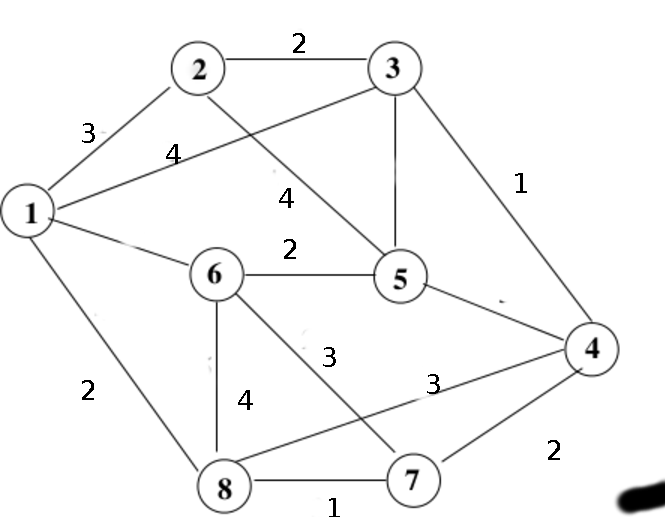
\includegraphics[width=2.7in]{edge_color_hw5.pdf}
\end{center}

\noindent
(a) For the graph above, find an edge
coloring with at most $4$ colors.

\medskip
\noindent
(b)
Let $\Delta$ denote the maximum vertex degree in a graph $G$.
Prove that if $\Delta\ge 1$ then $G$ can be edge-colored with
at most $2\Delta-1$ colors.
You need to give a direct proof, without using
any results from the literature.
Make your argument complete and rigorous.

\textbf{Problem 1B Solution}
\\*
Since $\Delta$ represents the maximum degree vertex in the graph, that means that we can color all edges with that same $\Delta$ colors.
\\*
The reason for this is that since we have at most $\Delta edges that are adjacent to eachother, therefore we need at least \Delta$ colors to make sure that no edge is the same color of any of its neighbours 
\\*
We want to show that $\Delta \leq 2*\Delta - 1$ because $\Delta \leq 1$, that means that $\Delta \leq 2*\Delta -1$ colors are sufficient to color the graph. 
\\*
There ends the proof.
\\*\\*
\smallskip
\emph{Hint:} In class we proved that each graph
of maximum degree $\Delta$ has a vertex coloring with at most
$\Delta+1$ colors. Follow the reasoning from that proof, modifying it slightly
to work for coloring edges.
\end{problem}

%%%%%%%%%%%%%%%%%%%%%%%%%%%%

\begin{problem}
Let $G$ be a planar graph with $n$ vertices and $m$ edges, where $n \ge 3$. 
Prove that if $G$ is bipartite then	$m \le 2n - 4$. 

\smallskip
\emph{Hint}: Follow the proof for Euler's inequality ($m \le 3n-6$) that 
	we covered in class. In that proof we used the equation 
$m = n + f - 2$, and to find a relationship between $m$ and $f$ we 
	estimated the number of ``edge sides" by $3f$, by noticing that
	each face must have at least three edge sides. How can you improve this
	estimate if $G$ is bipartite? Can a face of $G$ have three edges?
\end{problem}


\textbf{Problem 2 Solution}
\\*
In a bipartite planar graph, it is true that with $n \geq 3$ then it takes at least 2 added edges to create a face.
\\*
We can see that this is true for $m = 4$ because with 4 edges you can create no more than $\frac{4}{2}$ faces.
\\*
\\*Using this information, we can derive the inequality $2f \leq m$ where $f = $number of faces, and $m = $number of edges.
\\*
Simplifying the inequality gives: $f \leq \frac{m}{2}$
\\*
Simplifying Euler's formula gives: $f = m - n + 2$
\\*
Substituting our inequality into Euler's equation gives: $\frac{m}{2} \geq m - n + 2$
\\*
Simplification gives: $m \leq 2n - 4$ Which ends our proof.
\\*\\*
%%%%%%%%%%%%%%%%%%%%%%%%%%%%

\begin{problem}
Determine the minimum number of colors needed to color
the vertices of the following graph $G$:

\begin{center}
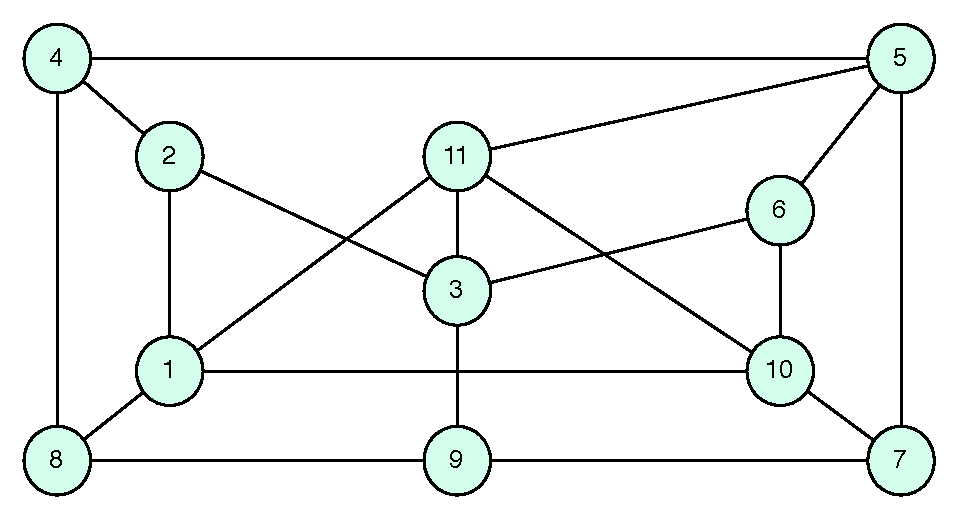
\includegraphics[width = 3in]{color_graph_hw5.pdf}
\end{center}

You need to (a) show a coloring with minimum number
of colors and (b) prove that it is not possible to
use fewer colors.
\end{problem}

%%%%%%%%%%%%%%%%%%%%%%%%%%%%



\vskip 0.1in
\paragraph{Submission.}
To submit the homework, you need to upload the pdf file into ilearn by 8AM on Friday, March 15,
and turn-in a paper copy in class.
Pictures should be 
imported into {\LaTeX} in pdf (see the source file to see
how to do that). You can draw them in any drawing
software and export in pdf, or draw by hand and scan.

\end{document}

